\section*{Abstract}\label{Abstract}
In diesem Projekt wird ein Logdatei-Parser erstellt, der eine Agilent-Logdatei einlesen und in ein gegebenes Zwischenformat umwandeln kann. Das Zwischenformat wird dabei nicht ausgeben, sondern nur im Hauptspeicher zur Verf�gung gestellt. Der Parser soll als eine Art Bibliothek von einem anderen Programmen genutzt werden, dass dieses Zwischenformat �bernimmt und weiterverarbeitet.

\begin{figure}[htp]
\centering
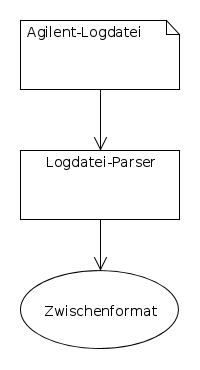
\includegraphics[width=0.3\textwidth]{Ingo/Bilder/Ablauf.png}
\caption{Ablauf}
\label{fig:Ablauf}
\end{figure}